Clase: 03/11/2022

\begin{lema}
    Sea $f(z)$ analítica en una región $A$ acotada por los círculos concéntricos $\gamma_1$ y $\gamma_2$. Si $z_0\in A$, entonces:
    \begin{align*}
        f(z_0) &= \int_{\gamma_1}\frac{f(z)}{z-z_0}dz-\int_{\gamma_2}\frac{f(z)}{z-z_0}dz
    \end{align*}
    \begin{dem}
        Sea 

        \begin{figure}[H]
            \centering
            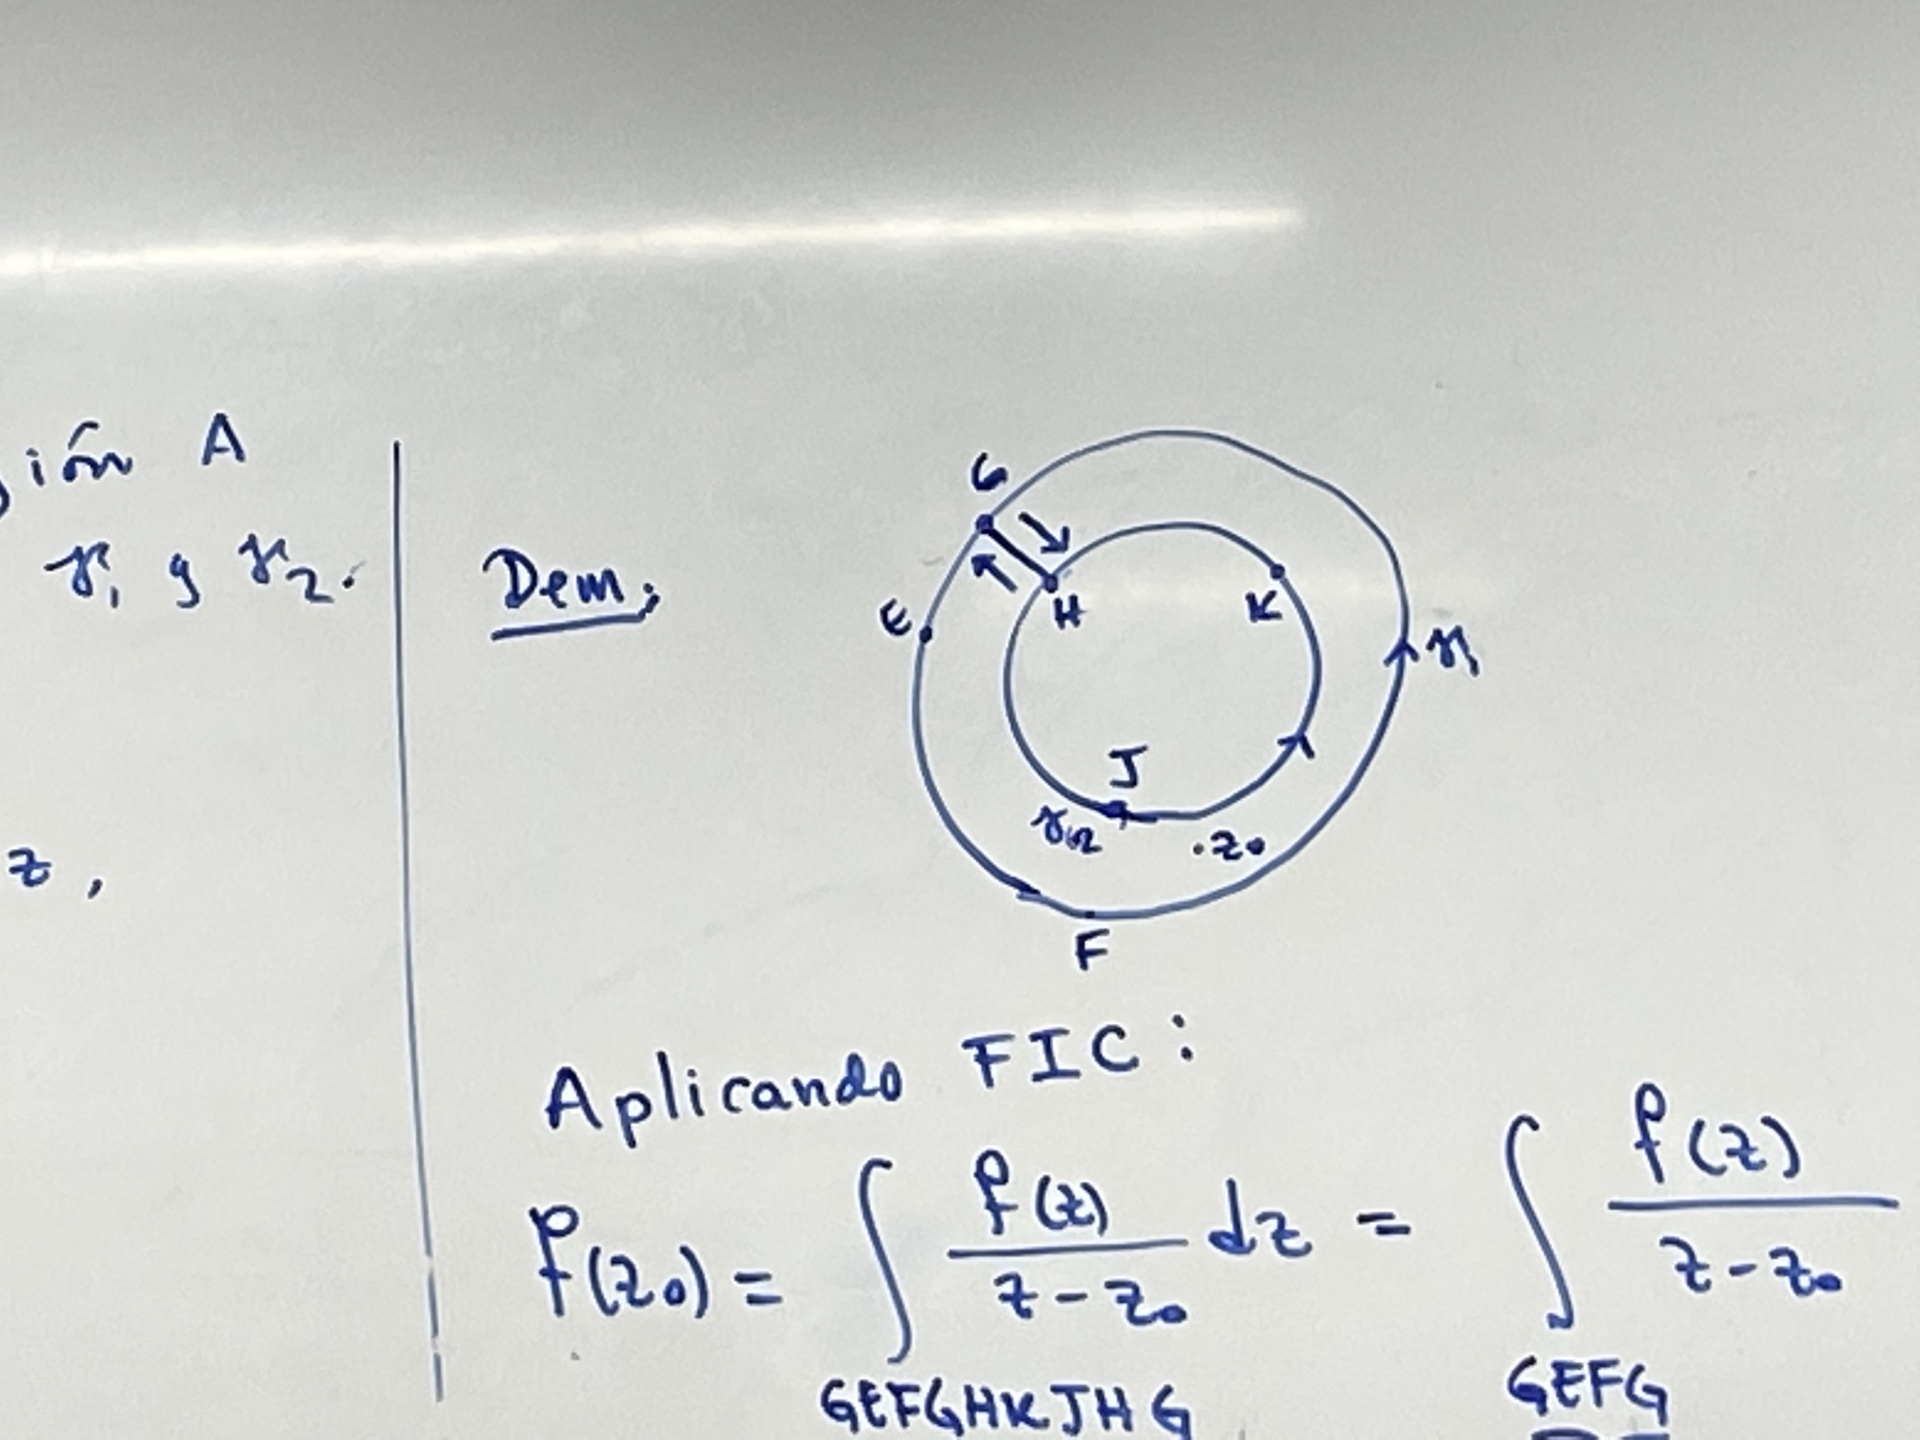
\includegraphics[scale=0.2]{imagenes/24.1.jpeg}
        \end{figure}
        Aplicando FIC: 
        \begin{align*}
            f(z_0) &= \int_{GEFGHJHG} \frac{f(z)}{z-z_0}dz\\
                   &= \int_{\underbrace{GEFG}_{\gamma_1}}\frac{f(z)}{z-z_0}dz+\int_{GH}\frac{f(z)}{z-z_0}dz+\int_{\underbrace{HKJH}_{-\gamma_2}}\frac{f(z)}{z-z_0}+\int_{HG}\frac{f(z)}{z-z_0}dz
        \end{align*}
    \end{dem}
\end{lema}

\begin{teorema}[Laurent]
    Sea $f$ analítica en la región $A$: 
    \begin{figure}[H]
        \centering
        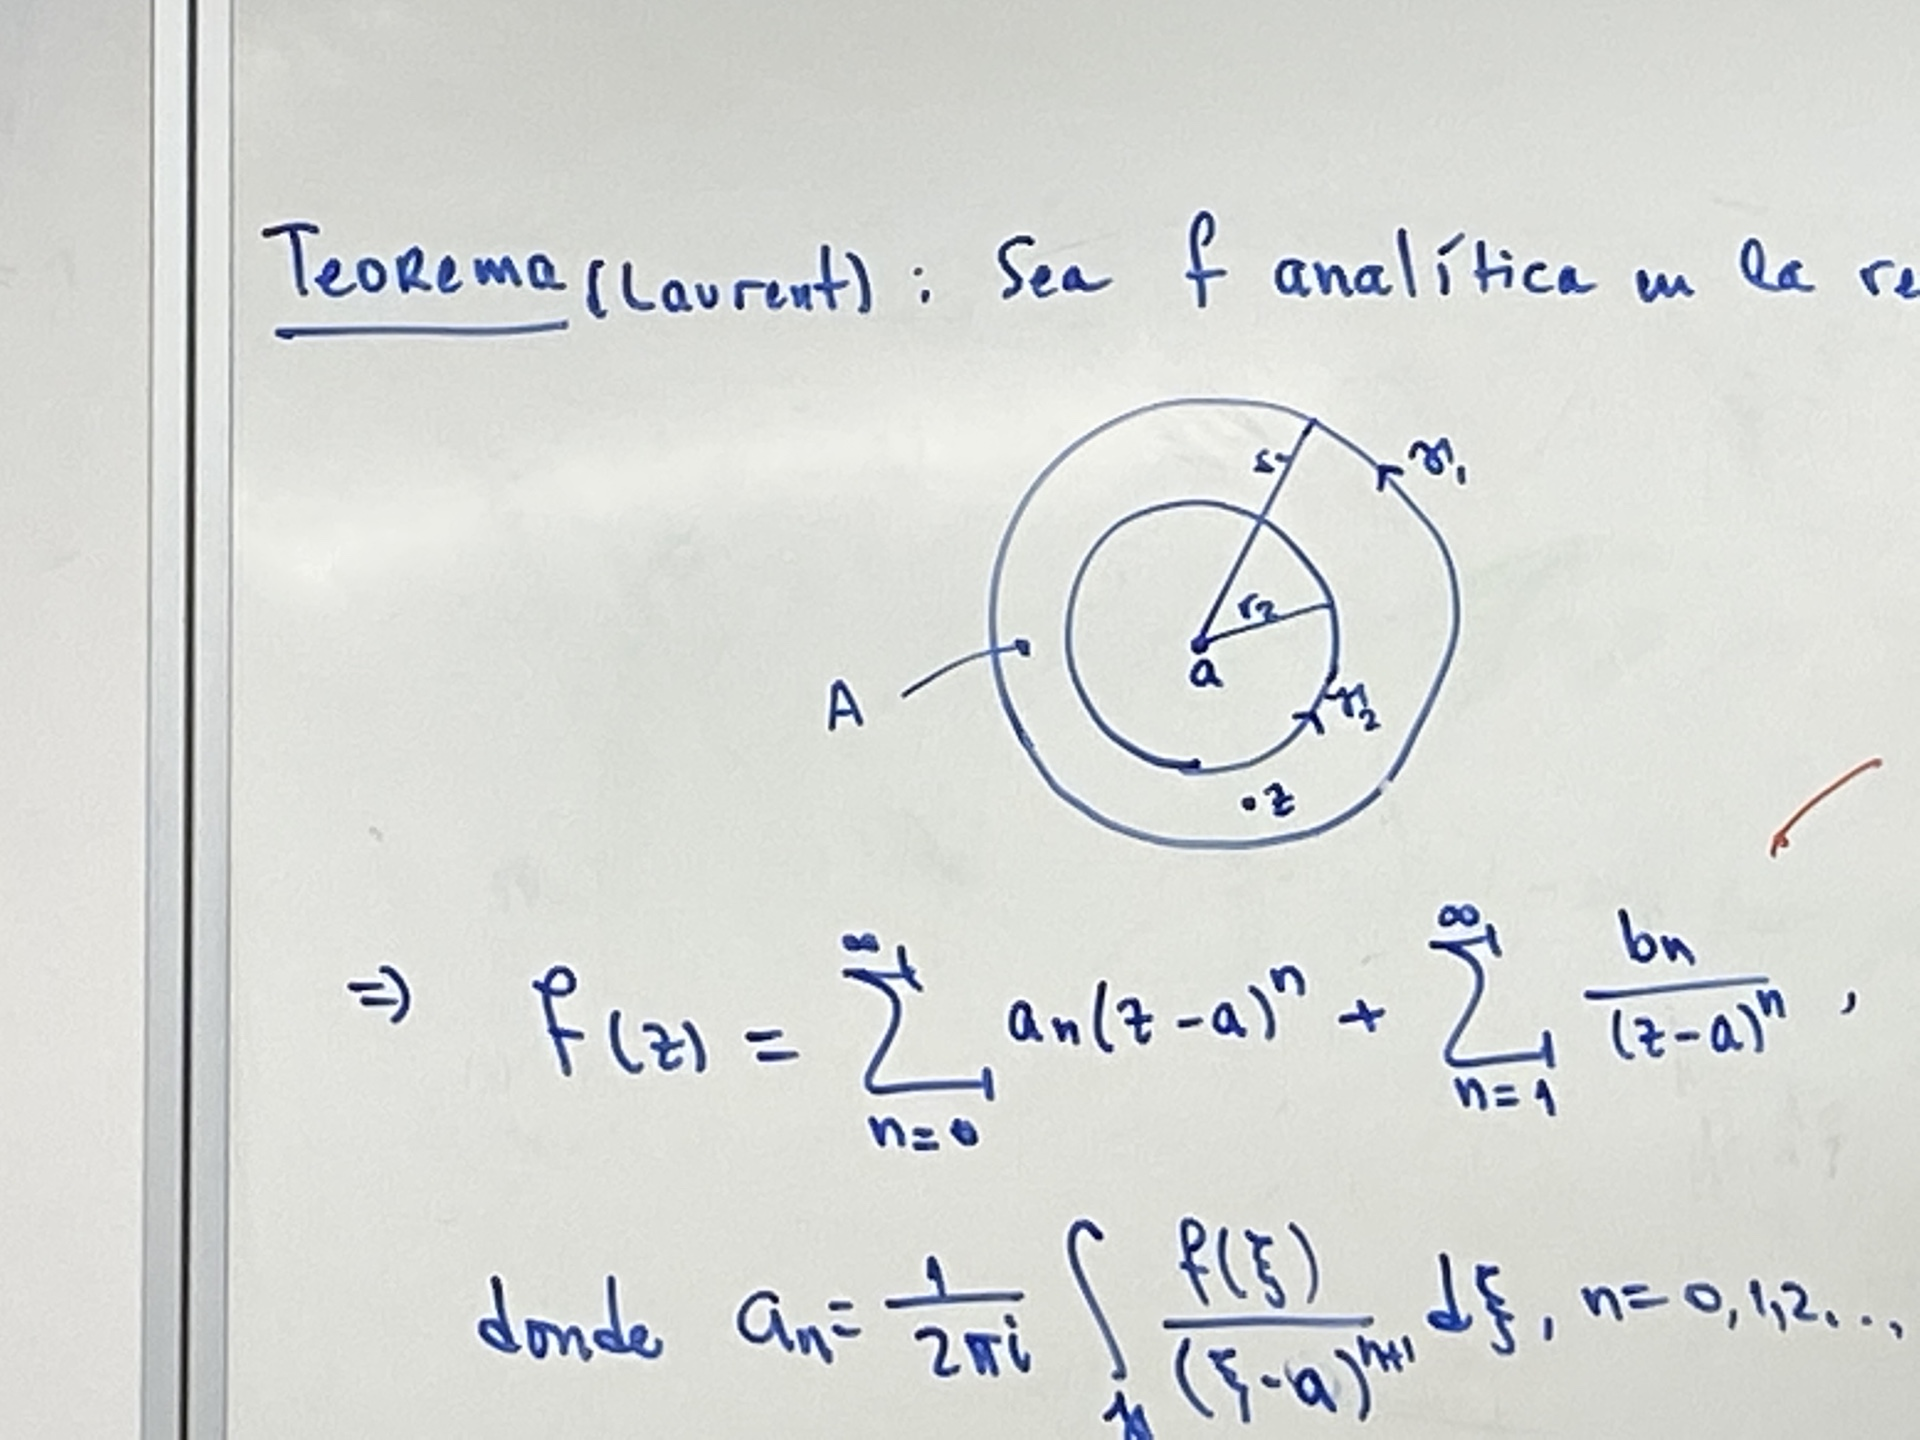
\includegraphics[scale=0.2]{imagenes/24.2.jpeg}
    \end{figure}
    \begin{align*}
        f(z)&=\sum_{n=1}^\infty a_n(z-a)^n +\sum_{n=1}^\infty \frac{b_n}{(z-a)^n}\\
        a_n &= \frac{1}{2\pi i}\int_{\gamma_1}\frac{f(\psi)}{(\psi-a)^{n+1}}d\psi, \quad n=0,1,2,\cdots\\
        b_n &= \frac{1}{2\pi i}\int_{\gamma_2}f(\psi)(\psi-a)^{n+1}d\psi, n=1,2,\cdots
    \end{align*}
    \begin{cajita}
        Tenemos 
        $$\sum_{n=-\infty}^\infty c_n(z-a)^n$$
    \end{cajita}
    \begin{dem}
        Por lema, 
        \begin{align*}
            f(z) &= \int_{\gamma_1}\frac{f(\psi)}{\psi -z}d\psi -\int_{\gamma_2}\frac{f(\psi)}{\psi-z}d\psi\\
        \end{align*}
        Para $\gamma_1$:
        \begin{align*}
            \frac{1}{\psi -a} &= \frac{1}{(\psi-a)-(z-a)}\\
            &= \frac{1}{(\psi -a)}\left[\frac{1}{1-\left(\frac{z-a}{\psi-a}\right)}\right]
            \intertext{Nótese que $\left|\frac{z-a}{\psi-a}\right|=\frac{|z-a|}{|\psi-a|}<1$}
        \end{align*}
        Entonces nótese que 
        \begin{align*}
           &\implies & 1+\left(\frac{z-a}{\psi-a}\right)+\left(\frac{z-a}{\psi-a}\right)^2+\cdots+\left(\frac{z-a}{\psi-a}\right)^{n-1} = \frac{1-\left(\frac{z-a}{\psi-a}\right)^n}{1-\left(\frac{z-a}{\psi -a}\right)}\\
            &\implies & \frac{1}{1-\frac{(z-a)}{(\psi-a)}} = 1+\left(\frac{z-a}{\psi-a}\right)+\cdots+\left(\frac{z-a}{\psi-a}\right)^{n-1}+\frac{1}{1-\left(\frac{z-a}{\psi-a}\right)}\left(\frac{z-a}{\psi-a}\right)^n\\
            &\implies& \frac{1}{\psi-z}= \frac{1}{\psi-a}+\frac{(z-a)}{(\psi-a)^2}+\cdots +\frac{(z-a)^{n-1}}{(\psi-a)^n}+\frac{1}{1-\left(\frac{z-a}{\psi-a}\right)}\cdot \frac{(z-a)^n}{(\psi-a)^{n+1}}
        \end{align*}
        Entonces 
        \begin{align*}
            \begin{split}
                \int_{\gamma_1}\frac{f(\psi)d\psi}{\psi -z} &= \int_{\gamma_1}\frac{f(\psi)d\psi}{\psi -a}+ \left[\int_{\gamma_2}\frac{f(\psi)}{(\psi-a)^2}d\psi\right](z-a)+\\
                &+ \left[\int_{\gamma_1}\frac{f(\psi)}{(\psi-a)^n}d\psi\right](z-a)^{n-1}+\underbrace{\int_{\psi_1}\frac{f(\psi)}{\psi-z}\left(\frac{z-a}{\psi-a}\right)^nd\psi}_{u_n}\\
                &= a_0(z-a)+a_2(z-a)^2+\cdots +a_{n-1}(z-a)^{n-1}+u_n
            \end{split}
        \end{align*}
        Para $\gamma_2:$
        \begin{align*}
            \frac{1}{\psi-z} = -\frac{1}{z-\psi} = -\frac{1}{(z-a)-(\psi-a)}=-\frac{1}{z-a}\left[\frac{1}{1-\frac{\psi-a}{z-a}}\right]
            \intertext{Nótese que $\left|\frac{z-a}{z-a}\right|<1$:}
            = -\left[\frac{1}{z-a}+\frac{(\psi -a)}{(z-a)^2}+\cdots + \frac{(\psi-a)^{n-1}}{(z-a){n}}+\frac{1}{1-\left(\frac{\psi-a}{z-a}\right)}\frac{(\psi-a)^n}{(z-a)^{n+1}}\right]
        \end{align*}
        Entonces
        \begin{align*}
            \int_{\gamma_2}\frac{f(\psi)}{(\psi -z)}d\psi &= -\left[\int_{\gamma_2}\frac{f(\psi)}{z-a}(\psi-a)d\psi+\cdots +\int_{\gamma_2}\frac{f(\psi)}{(z-a)^n}(\psi-a)^{n-1}d\psi\right. \\
            &\left.+\underbrace{\int_{\gamma_2}\frac{f(\psi)}{(z-a)^{n}}\cdot \frac{(\psi-a)^n}{z-\psi}d\psi}_{v_n}\right]
        \end{align*}
        Entonces, 
        $$f(z)=a_0+a_1(z-a)+\cdots+a_{n-1}(z-a)^{n-1}+u_n+\frac{b_1}{z-a}+\frac{b_2}{(z-a)^2}+\cdots + \frac{b_{n-1}}{(z-a)^n}+v_n$$

        A probar: $u_n\to_{n\to\infty}0$

        Tenemos que 
        $$|u_n|=\left|\int_{\gamma_1}\frac{f(\psi)}{\psi -z}\frac{(z-a)^n}{(\psi-a)^n}\right|\leq \frac{2\pi r_1\cdot \underbrace{|f(\psi)|}_{M}\lambda^n}{r_1-|z-a|}\to_{n\to \infty}0$$

        \begin{cajita}
            Sea $\lambda =\left|\frac{z-a}{\psi-a}\right|$, 
            en donde 
            $$|\psi -z| = |(\psi-a)-(z-a)|\geq |\psi-a|-|z-a|=r_1-|z-a|$$
        \end{cajita}
    \end{dem}
\end{teorema}

